\documentclass[tikz,border=10pt]{standalone}
\usepackage{amssymb} % For \S symbol
\usetikzlibrary{shapes.geometric}

\begin{document}
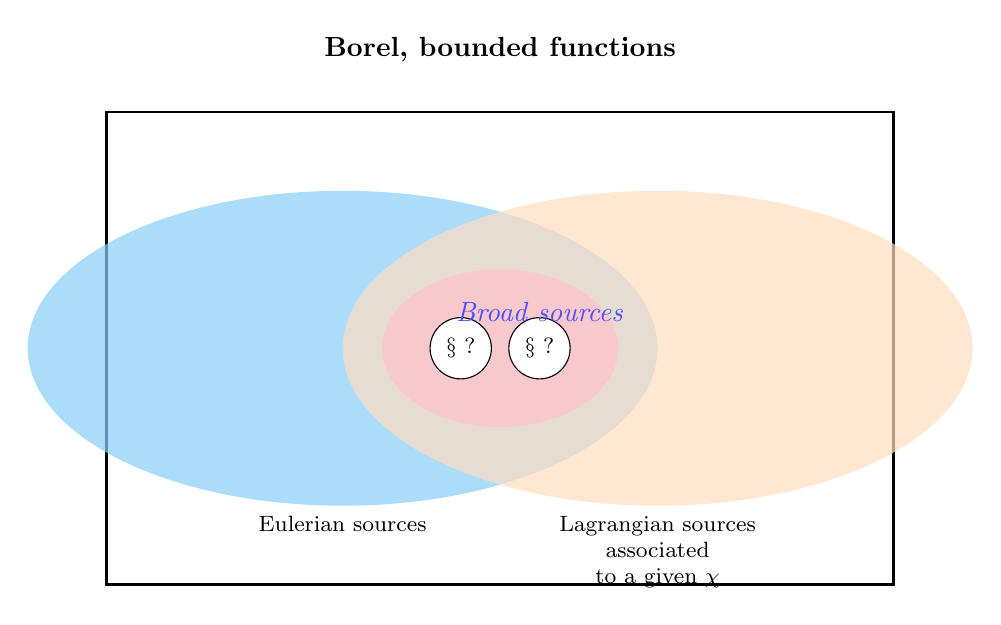
\begin{tikzpicture}[
    every node/.style={font=\footnotesize},
    set/.style={text width=2.5cm, align=center, anchor=north},
]

% Define colors for shading
\definecolor{eulerian}{RGB}{135,206,250}
\definecolor{lagrangian}{RGB}{255,221,191}
\definecolor{intersection}{RGB}{255,192,203}
\definecolor{borel}{RGB}{255,255,255}

% Draw the background box
\node[draw, rectangle, minimum width=10cm, minimum height=6cm, line width=1pt] (box) {};

% Draw the Eulerian sources ellipse
\node[ellipse, minimum width=8cm, minimum height=4cm, fill=eulerian, opacity=0.7, label={[set]below:Eulerian sources}] (eulerian) at (-2,0) {};

% Draw the Lagrangian sources ellipse
\node[ellipse, minimum width=8cm, minimum height=4cm, fill=lagrangian, opacity=0.7, label={[set]below:Lagrangian sources\\associated to a given $\chi$}] (lagrangian) at (2,0) {};

% Draw the intersection region
\node[ellipse, minimum width=3cm, minimum height=2cm, fill=intersection, opacity=0.7, anchor=center] (intersection) at (0,0) {};

% Draw the symbols and question marks inside the intersection
\node[circle, draw, fill=borel, minimum size=10pt, anchor=center] at (-0.5,0) {$\S~?$};
\node[circle, draw, fill=borel, minimum size=10pt, anchor=center] at (0.5,0) {$\S~?$};

% Add the "Broad sources" label
\node[anchor=north, text=blue!70, font=\itshape, shift={(0.5,-0.3)}] at (intersection.north) {Broad sources};

% Add the title
\node[anchor=south, font=\bfseries, shift={(0,0.5)}] at (box.north) {Borel, bounded functions};

\end{tikzpicture}
\end{document}